
\documentclass{standalone}

\usepackage{pgfplots}

\usepackage{tikz,amsmath, amssymb,bm,color}
\usepackage{graphicx, nicefrac}

\definecolor{darkbrown}{rgb}{0.4, 0.26, 0.13}

\definecolor{calpolypomonagreen}{rgb}{0.12, 0.3, 0.17}

\newcommand*{\Scale}[2][4]{\scalebox{#1}{$#2$}}%
\newcommand*{\Resize}[2]{\resizebox{#1}{!}{$#2$}}%
%\[y = \sin^2 x\]
%%
%\[\Scale[0.5]{y = \sin^2 x}\]
%%
%\[ \Resize{1cm}{y = \sin^2 x}\]


\begin{document}
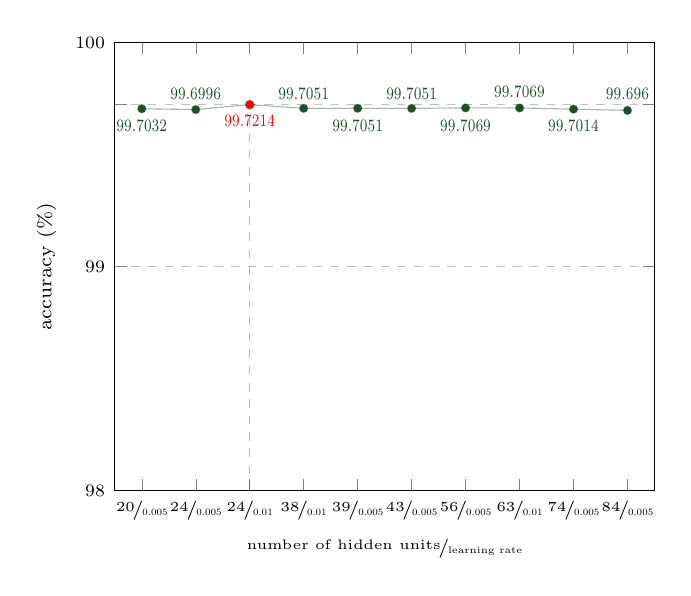
\begin{tikzpicture}
\begin{axis}[
	font = \scriptsize,
	xlabel=\nicefrac{number of hidden units}{\scalebox{0.7}[0.7]{learning rate}},
	ylabel=accuracy (\%),
	xmin=0.5, xmax=10.5,
	ymin=98, ymax=100,
	xtick={1, 2, 3, 4, 5, 6, 7, 8, 9, 10},
	ytick={98, 99, 99.7214, 100},
	xticklabels = {$\nicefrac{20}{\scalebox{0.5}[0.5]{0.005}}$, $\nicefrac{24}{\scalebox{0.5}[0.5]{0.005}}$, $\nicefrac{24}{\scalebox{0.5}[0.5]{0.01}}$, $\nicefrac{38}{\scalebox{0.5}[0.5]{0.01}}$, $\nicefrac{39}{\scalebox{0.5}[0.5]{0.005}}$, $\nicefrac{43}{\scalebox{0.5}[0.5]{0.005}}$, $\nicefrac{56}{\scalebox{0.5}[0.5]{0.005}}$, $\nicefrac{63}{\scalebox{0.5}[0.5]{0.01}}$, $\nicefrac{74}{\scalebox{0.5}[0.5]{0.005}}$, $\nicefrac{84}{\scalebox{0.5}[0.5]{0.005}}$},
	yticklabels = {\scalebox{0.9}[0.9]{98},\scalebox{0.9}[0.9]{99}, \scalebox{0.9}[0.9]{}, \scalebox{0.9}[0.9]{100}},
	ylabel near ticks,
    xlabel near ticks,
	legend pos=south west,
	legend style={mark size=2pt, font={\tiny \itshape}},
	ymajorgrids=true,
	grid style=dashed,
]
\addplot [mark=*, mark size=1.5pt, color = calpolypomonagreen ,draw opacity=0.4] coordinates {
	(1,99.7032)(2,99.6996)(3,99.7214)(4,99.7051)(5,99.7051)(6,99.7051)(7,99.7069)(8,99.7069)(9,99.7014)(10,99.696)
};

\addplot [mark=*, mark size=1.5pt, color = red ,draw opacity=0.4] coordinates {
	(3,99.7214)
};
\addplot [dashed, red, draw opacity=0.4] coordinates {(3,0)(3,99.7214)};
\node[calpolypomonagreen, font=\scriptsize] at (axis cs: 10,99.77) {\scalebox{0.7}[0.9]{99.696}};

\node[calpolypomonagreen, font=\scriptsize] at (axis cs: 9,99.63) {\scalebox{0.7}[0.9]{99.7014}};

\node[calpolypomonagreen, font=\scriptsize] at (axis cs: 8,99.78) {\scalebox{0.7}[0.9]{99.7069}};

\node[calpolypomonagreen, font=\scriptsize] at (axis cs: 7,99.63) {\scalebox{0.7}[0.9]{99.7069}};

\node[calpolypomonagreen, font=\scriptsize] at (axis cs: 6,99.77) {\scalebox{0.7}[0.9]{99.7051}};

\node[calpolypomonagreen, font=\scriptsize] at (axis cs: 5,99.63) {\scalebox{0.7}[0.9]{99.7051}};

\node[calpolypomonagreen, font=\scriptsize] at (axis cs: 4,99.77) {\scalebox{0.7}[0.9]{99.7051}};

\node[red, font=\scriptsize] at (axis cs: 3,99.65) {\scalebox{0.7}[0.9]{99.7214}};

\node[calpolypomonagreen, font=\scriptsize] at (axis cs: 2,99.77) {\scalebox{0.7}[0.9]{99.6996}};

\node[calpolypomonagreen, font=\scriptsize] at (axis cs: 1,99.63) {\scalebox{0.7}[0.9]{99.7032}};



%\legend{LGBM,RF,XGB}
\end{axis}
\end{tikzpicture}
\end{document}
